\documentclass[12pt]{standalone}
\usepackage{tikz}
%\usetikzlibrary{calc, arrows.meta, decorations.pathreplacing}

\begin{document}

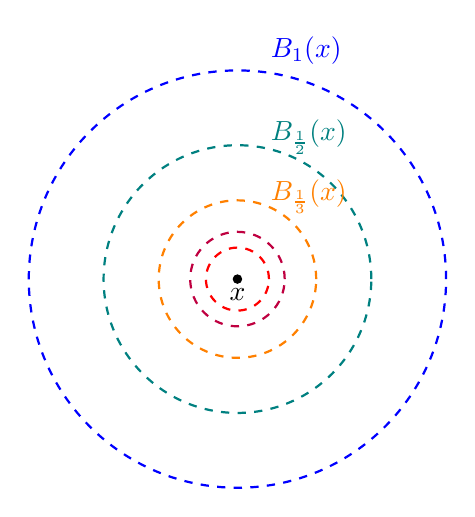
\begin{tikzpicture}[scale=1]
  \coordinate (x) at (0,0);

  \draw[blue, thick, dashed] (x) circle (2.65);
  \draw[teal, thick, dashed] (x) circle (1.7);
  \draw[orange, thick, dashed] (x) circle (1.0);
  \draw[purple, thick, dashed] (x) circle (0.6);
  \draw[red, thick, dashed] (x) circle (0.4);

  \node[blue, anchor=west] at (0.3,2.9) {$B_1(x)$};
  \node[teal, anchor=west] at (0.3,1.8) {$B_{\frac12}(x)$};
  \node[orange, anchor=west] at (0.3,1.05) {$B_{\frac13}(x)$};
  % \node[purple, anchor=west] at (0.75,0.1) {$B_{1/4}(x)$};
  % \node at (0.12,0.42) {$\cdots$};

  \filldraw[black] (x) circle (1.5pt) node[below] {$x$};

  % \node at (0,-2.9) {$\displaystyle \bigcap_{n=1}^{\infty} B_{1/n}(x)=\{x\}$};
\end{tikzpicture}

\end{document}
